\section{Initial System Design}

Come up with this myself and read little of other peoples designs. Wickerson said he was a proponent of the philosophy of doing it from scratch. The design will be bad but it will be a more interesting learning process for me and I might come up with some different ideas. Gives me the opportunity to design something ground up and compare with other peoples designs at the end of the project.

Sounds more fun in general.

In this section, I propose an initial design for the overall system and the important subsystems. Arrows in each of the figures in this section represent the direction of data flow in the design. \Cref{fig:SysMemShared} shows a very simple design for the overall system architecture. 
The Rasterizer hardware receives input from the CPU Core. This will be control and data input. The data input will be the register contents of the registers being used as input in the instruction. The control input is used by the CPU to tell the rasterizer when it can start processing data from memory. This will likely trigger on the completion of the preceding fence instruction.  
The CPU and rasterizer will also have direct access to memory for reading and writing to and from memory. 

The memory hierarchy of the CPU will need to be decided on at a later date. 

\begin{figure}[ht]
    \centering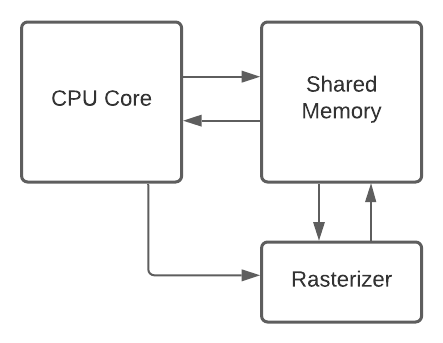
\includegraphics[width=6cm]{functional_spec/images/SysMemShared.png}
    \caption{Caption text 1}
    \label{fig:SysMemShared}
\end{figure}

\begin{landscape}
    \begin{figure}[ht]
        \centering
        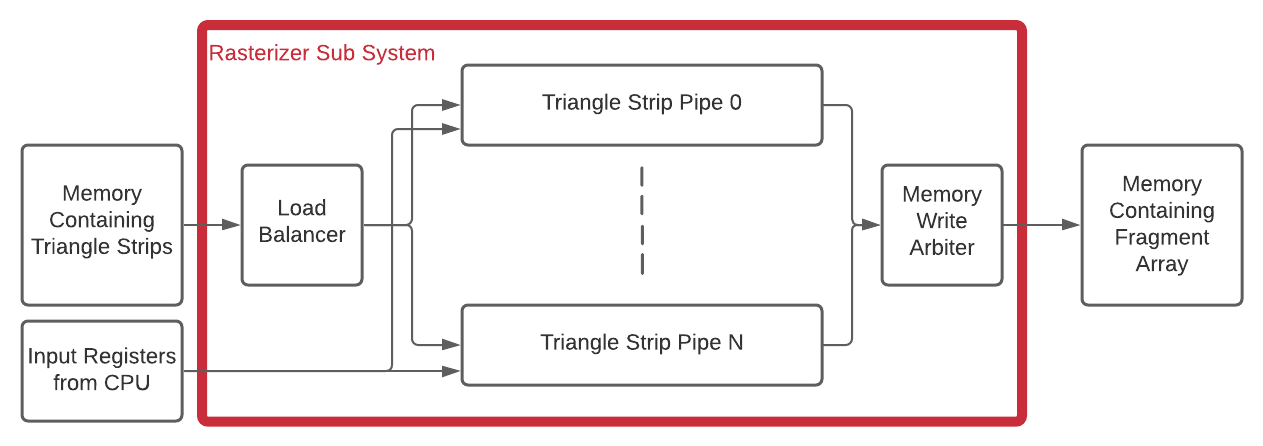
\includegraphics[width=19cm]{functional_spec/images/RasterizerSS.png}
        \caption{Caption}
        \label{fig:RasterizerSS}
    \end{figure}
\end{landscape}
\begin{landscape}
    \begin{figure}[ht]
        \centering
        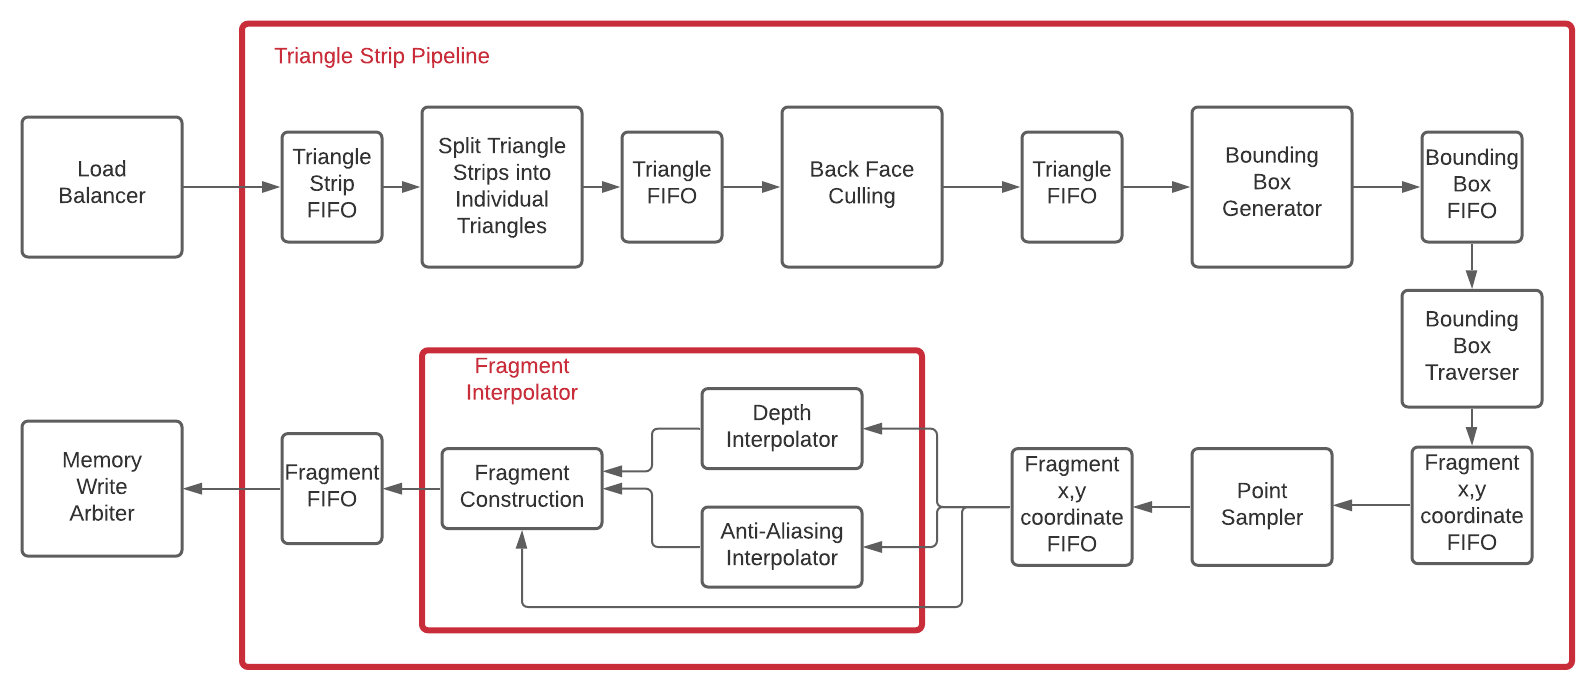
\includegraphics[width=20cm]{functional_spec/images/TriangleStripPipe.png}
        \caption{Caption}
        \label{fig:TriangleStripPipe}
    \end{figure}\end{landscape}

